% SIAM Article - HRP Portfolio Optimization with Regime-Based Enhancement
\documentclass[review,onefignum,onetabnum]{siamart171218}

\usepackage{amsmath,amssymb,amsfonts}
\usepackage{graphicx}
\usepackage{booktabs}
\usepackage{algorithm}
\usepackage{algorithmic}
\usepackage{hyperref}
\usepackage{cleveref}
\usepackage{titlesec}

% TikZ for diagrams
\usepackage{tikz}
\usetikzlibrary{shapes.geometric, arrows.meta, positioning, calc, backgrounds, fit, decorations.pathreplacing}

% ============================================================================
% FORMATTING: Centered titles and increased spacing
% ============================================================================

% Only number sections and subsections (not subsubsections)
\setcounter{secnumdepth}{2}

% Left-aligned section titles
\titleformat{\section}
  {\normalfont\Large\bfseries}{\thesection.}{1em}{}
\titleformat{\subsection}
  {\normalfont\large\bfseries}{\thesubsection.}{1em}{}
% Subsubsections: bold, left-aligned, but NO number
\titleformat{\subsubsection}
  {\normalfont\normalsize\bfseries}{}{0em}{}

% Add spacing before and after sections
\titlespacing*{\section}{0pt}{2.5ex plus 1ex minus .2ex}{1.5ex plus .2ex}
\titlespacing*{\subsection}{0pt}{2ex plus 1ex minus .2ex}{1ex plus .2ex}
\titlespacing*{\subsubsection}{0pt}{1.5ex plus 1ex minus .2ex}{0.8ex plus .2ex}

% Increase paragraph spacing
\setlength{\parskip}{0.8em plus 0.1em minus 0.1em}

% Slightly increase line spacing for readability
\linespread{1.1}

% ============================================================================

% Custom commands
\newcommand{\E}{\mathbb{E}}
\newcommand{\R}{\mathbb{R}}
\newcommand{\bx}{\mathbf{x}}
\newcommand{\bw}{\mathbf{w}}

% ============================================================================
% TikZ Style Definitions for Pipeline Diagrams
% ============================================================================
\tikzstyle{databox} = [rectangle, rounded corners, minimum width=2cm, minimum height=0.8cm, 
                       text centered, draw=blue!70, fill=blue!10, font=\small]
\tikzstyle{processbox} = [rectangle, rounded corners, minimum width=2cm, minimum height=0.8cm,
                          text centered, draw=orange!70, fill=orange!10, font=\small]
\tikzstyle{outputbox} = [rectangle, rounded corners, minimum width=2cm, minimum height=0.8cm,
                         text centered, draw=green!70, fill=green!20, font=\small]
\tikzstyle{mlbox} = [rectangle, rounded corners, minimum width=2cm, minimum height=0.8cm,
                     text centered, draw=purple!70, fill=purple!10, font=\small]
\tikzstyle{arrow} = [thick, ->, >=Stealth]
\tikzstyle{doublearrow} = [thick, <->, >=Stealth]
\tikzstyle{phasebox} = [rectangle, rounded corners, minimum width=2.5cm, minimum height=1cm,
                        text centered, draw=black!50, fill=white, font=\small, text width=2.3cm]
\tikzstyle{timeblock} = [rectangle, minimum width=1.5cm, minimum height=0.6cm, 
                         text centered, font=\scriptsize]

% PDF metadata
\ifpdf
\hypersetup{
  pdftitle={Regime-Adaptive Hierarchical Risk Parity: A Machine Learning Approach to Dynamic Portfolio Allocation},
  pdfauthor={Lucas Jaccard}
}
\fi

\begin{document}

\title{Regime-Adaptive Hierarchical Risk Parity: A Machine Learning Approach to Dynamic Portfolio Allocation}

\author{Lucas Jaccard\thanks{Master of Finance (HEC Lausanne), Advanced Data Analysis Course, January 2026.}}

\maketitle

%==============================================================================
% ABSTRACT
%==============================================================================
\begin{abstract}
This paper presents a regime-adaptive portfolio framework combining Hierarchical Risk Parity (HRP) with Hidden Markov Model (HMM) regime detection and XGBoost prediction. Using CRSP data (1965--2024), a GPU-accelerated HRP portfolio is constructed with RMT denoising and a forward-only HMM filter using log returns, downside deviation, and Michigan Consumer Sentiment. The regime-adaptive strategy achieves a Sharpe ratio of 0.85 vs.\ 0.51 for static HRP and 0.54 for the market, after transaction costs. Critically, maximum drawdown falls from 45.7\% to 21.0\%, with all five worst drawdowns ($-$21.0\% to $-$13.5\%) smaller than static HRP's \textit{fifth} worst ($-$22.3\%). The XGBoost model achieves 66.2\% accuracy with 72.9\% bear recall out-of-sample.
\end{abstract}

%==============================================================================
% 1. INTRODUCTION
%==============================================================================
\section{Introduction}
\label{sec:intro}

In 1952, Harry Markowitz introduced Modern Portfolio Theory to the world and revolutionized the way portfolio managers allocate capital \cite{markowitz1952}. Most subsequent models and theories stem from this foundational work and its method for solving portfolio weights to minimize risk given a target return---or simply minimizing risk as a primary objective (the Global Minimum Variance Portfolio). Despite the elegance of its solution, several problems arise: How can the expected return vector be estimated reliably? How should the covariance matrix be inverted given a large number of assets? What is the appropriate risk aversion coefficient for a given investor?

While these questions were partially addressed in subsequent decades, the inversion of the covariance matrix remains problematic: it magnifies estimation errors at best, and sometimes the matrix cannot even be inverted due to singularity \cite{michaud1989}. Almost seventy years after Markowitz, in the paper ``Building Diversified Portfolios that Outperform Out-of-Sample,'' Marcos López de Prado proposed a machine learning framework---Hierarchical Risk Parity (HRP)---that does not require covariance matrix inversion to minimize risk \cite{lopez2016}. His methodology demonstrated less concentration in portfolio composition as well as reduced out-of-sample volatility and drawdown compared to mean-variance optimization.

The current paper aspires to address a problem that both of these methodologies face: the assumption of stationary market conditions.

%==============================================================================
% 2. RESEARCH QUESTION & LITERATURE
%==============================================================================
\section{Research Question \& Literature}
\label{sec:research}

Several assumptions in portfolio optimization are so widely accepted that they are rarely questioned:

\paragraph{Is variance the right metric to minimize?}
Most investors would gladly accept upside volatility---it is the \textit{downside} that destroys wealth. Fishburn \cite{fishburn1977} formalized this asymmetry with lower partial moments (LPM), showing that mean-variance optimization is merely a special case of a broader framework that penalizes only below-target returns. A 50\% loss requires a 100\% gain just to break even; a 20\% loss requires only 25\%. This mathematical and psychological asymmetry suggests that drawdown reduction may be more valuable than variance reduction.

\paragraph{Are correlations reliable when they matter most?}
Longin and Solnik \cite{longin2001} highlight a critical property of equity markets: correlations increase dramatically during market stress. In other words, estimated correlations become unreliable precisely when diversification is most needed. Ang and Bekaert \cite{ang2002} further develop the relationship between correlation spikes and drawdowns in diversified holdings, showing that regime-switching models can capture these dynamics.

\paragraph{Research Question.}
These observations motivate a natural question: \textit{Can portfolio construction capture the benefits of diversification in calm markets while dynamically reducing exposure before drawdowns materialize?}

\paragraph{Contributions.}
This work makes four contributions: (1) GPU-accelerated HRP with Random Matrix Theory denoising following Marchenko and Pastur \cite{marchenko1967} and Laloux et al.\ \cite{laloux1999}; (2) A forward-only HMM filter that avoids look-ahead bias from standard smoothed posteriors as in Hamilton \cite{hamilton1989}, combined with XGBoost (Chen and Guestrin \cite{chen2016}) for regime prediction; (3) Walk-forward backtesting with purged cross-validation following L\'opez de Prado \cite{lopez2018}; (4) Empirical evidence that drawdown reduction---not Sharpe ratio improvement---is the primary achievement.

\paragraph{Related Work.}
HRP was extended to multi-period settings by Raffinot \cite{raffinot2018}. Regime-switching models for asset allocation were studied by Ang and Bekaert \cite{ang2002} and Guidolin and Timmermann \cite{guidolin2007}. Machine learning for return prediction was surveyed by Gu, Kelly, and Xiu \cite{gu2020}. Consumer sentiment as a market predictor was examined by Lemmon and Portniaguina \cite{lemmon2006}. This work bridges HRP and ML-based regime prediction---a gap in the existing literature.

%==============================================================================
% 3. METHODOLOGY
%==============================================================================
\section{Methodology}
\label{sec:methodology}

The methodology consists of two parts: (1) the base HRP portfolio construction with RMT denoising, and (2) the regime-adaptive enhancement using HMM and XGBoost. This section presents a detailed 7-stage pipeline for Part 1 and a 6-phase pipeline for Part 2.

\subsection{Part 1: Hierarchical Risk Parity}

The HRP weight computation follows a 7-stage pipeline executed at each monthly rebalancing date. \Cref{fig:hrp-pipeline} provides a visual overview of this process.

\begin{figure}[htbp]
\centering
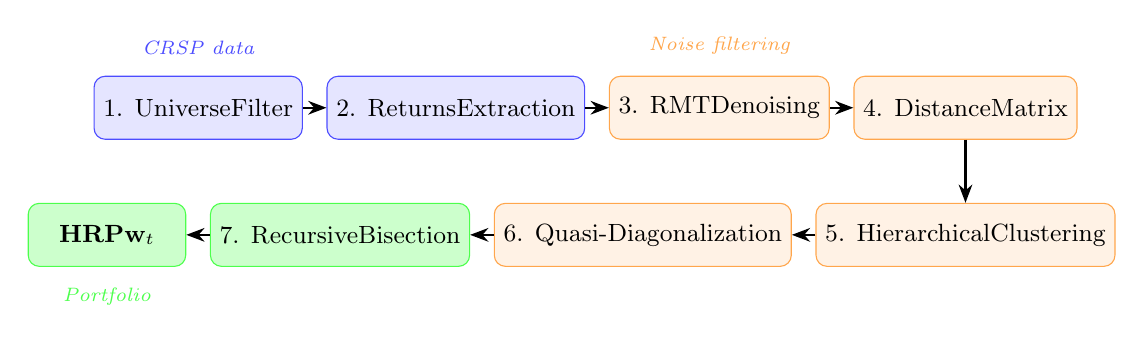
\begin{tikzpicture}[node distance=0.4cm and 0.3cm]
    % Row 1: Data Preparation
    \node[databox] (universe) {1. Universe\\Filter};
    \node[databox, right=of universe] (returns) {2. Returns\\Extraction};
    \node[processbox, right=of returns] (rmt) {3. RMT\\Denoising};
    \node[processbox, right=of rmt] (distance) {4. Distance\\Matrix};
    
    % Row 2: Clustering and Output
    \node[processbox, below=0.8cm of distance] (cluster) {5. Hierarchical\\Clustering};
    \node[processbox, left=of cluster] (seriation) {6. Quasi-\\Diagonalization};
    \node[outputbox, left=of seriation] (bisection) {7. Recursive\\Bisection};
    \node[outputbox, left=of bisection] (weights) {\textbf{HRP}\\$\mathbf{w}_t$};
    
    % Arrows Row 1
    \draw[arrow] (universe) -- (returns);
    \draw[arrow] (returns) -- (rmt);
    \draw[arrow] (rmt) -- (distance);
    
    % Arrow down
    \draw[arrow] (distance) -- (cluster);
    
    % Arrows Row 2
    \draw[arrow] (cluster) -- (seriation);
    \draw[arrow] (seriation) -- (bisection);
    \draw[arrow] (bisection) -- (weights);
    
    % Labels
    \node[above=0.15cm of universe, font=\scriptsize\itshape, text=blue!70] {CRSP data};
    \node[above=0.15cm of rmt, font=\scriptsize\itshape, text=orange!70] {Noise filtering};
    \node[below=0.15cm of weights, font=\scriptsize\itshape, text=green!70] {Portfolio};
\end{tikzpicture}
\caption{HRP 7-Stage Pipeline. Blue boxes represent data inputs, orange boxes represent transformations, and green boxes represent outputs. The pipeline flows from raw CRSP data through RMT denoising, hierarchical clustering, and recursive bisection to produce final portfolio weights.}
\label{fig:hrp-pipeline}
\end{figure}

\subsubsection{Stage 1: Universe Construction}
At each rebalancing date $t$, the investable universe is constructed from CRSP common shares (SHRCD $\in \{10, 11\}$) listed on NYSE, NASDAQ, or AMEX (EXCHCD $\in \{1, 2, 3\}$). A two-stage liquidity filter is then applied within each Fama-French 12 industry classification:
\begin{equation}
    \mathcal{U}_t = \left\{ i : V^{med}_{i,t} \geq Q_{80\%}(V^{med}_{ind(i),t}) \text{ and } P_{i,t} > \$3 \right\}
\end{equation}
where $V^{med}_{i,t}$ is the rolling 12-month median dollar volume (with minimum 6 valid observations), and $Q_{80\%}$ denotes the 80th percentile within each industry. This selects the top 20\% most liquid stocks per industry while excluding penny stocks.

\subsubsection{Stage 2: Return Extraction}
For each rebalancing date $t$, a 60-month ($T=60$) lookback window of returns is extracted for $N$ stocks passing the universe filter. Only stocks with all 60 monthly returns available are included:
\begin{equation}
    \mathbf{R}_{t} \in \mathbb{R}^{T \times N}, \quad \text{where } R_{s,i} = r_{i,s} \text{ for } s \in [t-59, t]
\end{equation}

\subsubsection{Stage 3: RMT Covariance Denoising}
Sample covariance matrices are notoriously noisy when $N$ approaches $T$. Random Matrix Theory (RMT) denoising is applied following Laloux et al.\ \cite{laloux1999}:

\paragraph{Step 3a: Decomposition.} Convert the covariance matrix to a correlation matrix $\mathbf{C}$ while preserving individual volatilities $\sigma_i$.

\paragraph{Step 3b: Eigendecomposition.}
\begin{equation}
    \mathbf{C} = \mathbf{V} \boldsymbol{\Lambda} \mathbf{V}^\top, \quad \boldsymbol{\Lambda} = \text{diag}(\lambda_1, \ldots, \lambda_N)
\end{equation}

\paragraph{Step 3c: Marchenko-Pastur Threshold.} The threshold separating signal from noise eigenvalues is:
\begin{equation}
    \lambda_{\max} = \hat{\sigma}^2 \left(1 + \sqrt{\frac{N}{T}}\right)^2
\end{equation}
where $\hat{\sigma}^2 = \text{median}(\lambda_1, \ldots, \lambda_N)$ is a robust estimator of the noise variance (Laloux et al.\ \cite{laloux1999}).

\paragraph{Step 3d: Denoising.} Eigenvalues below $\lambda_{\max}$ are replaced with their mean:
\begin{equation}
    \tilde{\lambda}_k = \begin{cases}
        \lambda_k & \text{if } \lambda_k > \lambda_{\max} \text{ (signal)} \\
        \bar{\lambda}_{noise} & \text{otherwise (noise)}
    \end{cases}
\end{equation}

\paragraph{Step 3e: Reconstruction.} The denoised correlation matrix is reconstructed as $\tilde{\mathbf{C}} = \mathbf{V} \tilde{\boldsymbol{\Lambda}} \mathbf{V}^\top$, then converted back to covariance: $\tilde{\boldsymbol{\Sigma}} = \text{diag}(\boldsymbol{\sigma}) \cdot \tilde{\mathbf{C}} \cdot \text{diag}(\boldsymbol{\sigma})$.

\subsubsection{Stage 4: Distance Matrix Construction}
The denoised correlation matrix is converted to a distance matrix using a two-step process following L\'opez de Prado \cite{lopez2016}:

\paragraph{Step 4a: Correlation Distance.} First, the angular distance between each pair of assets is computed:
\begin{equation}
    d_{i,j} = \sqrt{\frac{1}{2}(1 - \rho_{i,j})} \in [0, 1]
\end{equation}
This maps perfect correlation ($\rho=1$) to zero distance and perfect anti-correlation ($\rho=-1$) to maximum distance.

\paragraph{Step 4b: Euclidean Distance on Correlation Profiles.} Second, the Euclidean distance between each asset's correlation profile (i.e., its row in the distance matrix) is computed:
\begin{equation}
    \tilde{d}_{i,j} = \sqrt{\sum_{k=1}^{N} (d_{k,i} - d_{k,j})^2}
\end{equation}
This captures how similarly two assets correlate with the \textit{entire universe}. Two assets may have similar pairwise correlation but very different correlation patterns with other assets; this step distinguishes them.

\subsubsection{Stage 5: Hierarchical Clustering}
Ward's method \cite{ward1963} performs agglomerative clustering by iteratively merging the pair of clusters that minimizes the increase in total within-cluster variance:
\begin{equation}
    \Delta(A, B) = \frac{n_A n_B}{n_A + n_B} \| \bar{d}_A - \bar{d}_B \|^2
\end{equation}
The output is a dendrogram (binary tree) representing the hierarchical structure of asset similarities.

\subsubsection{Stage 6: Quasi-Diagonalization (Seriation)}
The dendrogram is reordered so that similar assets are placed adjacent, producing a quasi-diagonal covariance matrix. This seriation step traverses the tree and orders leaves such that the largest cluster elements appear first, creating a banded structure that facilitates the recursive bisection.

\subsubsection{Stage 7: Recursive Bisection}
Weights are allocated through top-down recursive bisection of the seriated dendrogram. At each node splitting cluster $C$ into $C_1$ and $C_2$:
\begin{equation}
    \alpha = 1 - \frac{\tilde{V}_{C_1}}{\tilde{V}_{C_1} + \tilde{V}_{C_2}}, \quad w_{C_1} = \alpha \cdot w_C, \quad w_{C_2} = (1-\alpha) \cdot w_C
\end{equation}
where $\tilde{V}_C$ is the cluster variance computed as an inverse-variance portfolio:
\begin{equation}
    \tilde{V}_C = \left( \sum_{i \in C} \frac{1}{\sigma_i^2} \right)^{-1} \cdot \mathbf{1}^\top \boldsymbol{\Sigma}_C^{-1} \mathbf{1}
\end{equation}
This allocates more weight to the lower-variance branch at each split, producing a risk-balanced portfolio without matrix inversion of the full covariance matrix.

\subsection{Part 2: Regime-Adaptive Enhancement}

The regime-adaptive enhancement follows a 6-phase pipeline that predicts market regimes and adjusts portfolio exposure accordingly. \Cref{fig:ml-pipeline} illustrates the complete workflow.

\begin{figure}[htbp]
\centering
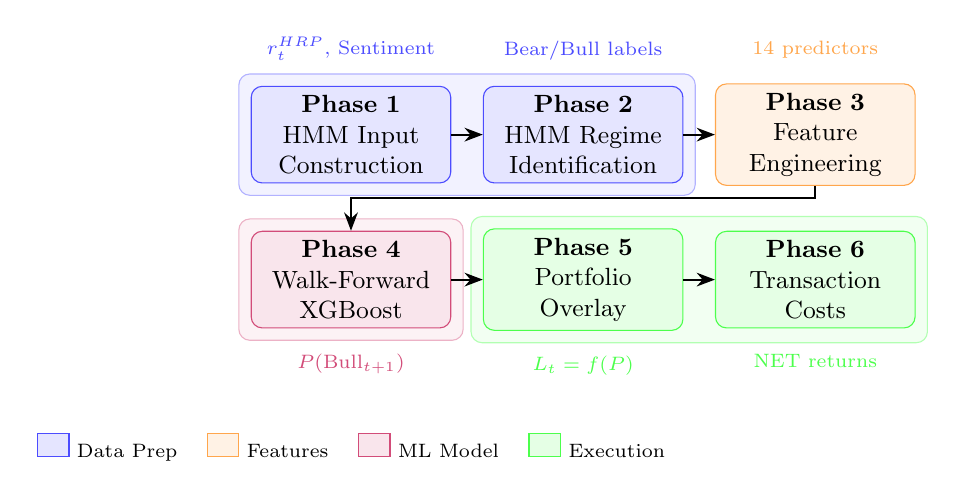
\begin{tikzpicture}[node distance=0.15cm]
    % Phase boxes - two rows
    \node[phasebox, fill=blue!10, draw=blue!70] (p1) {\textbf{Phase 1}\\HMM Input\\Construction};
    \node[phasebox, fill=blue!10, draw=blue!70, right=0.4cm of p1] (p2) {\textbf{Phase 2}\\HMM Regime\\Identification};
    \node[phasebox, fill=orange!10, draw=orange!70, right=0.4cm of p2] (p3) {\textbf{Phase 3}\\Feature\\Engineering};
    
    \node[phasebox, fill=purple!10, draw=purple!70, below=0.6cm of p1] (p4) {\textbf{Phase 4}\\Walk-Forward\\XGBoost};
    \node[phasebox, fill=green!10, draw=green!70, right=0.4cm of p4] (p5) {\textbf{Phase 5}\\Portfolio\\Overlay};
    \node[phasebox, fill=green!10, draw=green!70, right=0.4cm of p5] (p6) {\textbf{Phase 6}\\Transaction\\Costs};
    
    % Arrows
    \draw[arrow] (p1) -- (p2);
    \draw[arrow] (p2) -- (p3);
    \draw[arrow] (p3) -- ++(0,-0.8cm) -| (p4);
    \draw[arrow] (p4) -- (p5);
    \draw[arrow] (p5) -- (p6);
    
    % Input/Output annotations
    \node[above=0.2cm of p1, font=\scriptsize, text=blue!70] {$r_t^{HRP}$, Sentiment};
    \node[above=0.2cm of p2, font=\scriptsize, text=blue!70] {Bear/Bull labels};
    \node[above=0.2cm of p3, font=\scriptsize, text=orange!70] {14 predictors};
    \node[below=0.2cm of p4, font=\scriptsize, text=purple!70] {$P(\text{Bull}_{t+1})$};
    \node[below=0.2cm of p5, font=\scriptsize, text=green!70] {$L_t = f(P)$};
    \node[below=0.2cm of p6, font=\scriptsize, text=green!70] {NET returns};
    
    % Background groupings
    \begin{scope}[on background layer]
        \node[fit=(p1)(p2), rounded corners, draw=blue!30, fill=blue!5, inner sep=0.15cm] {};
        \node[fit=(p4), rounded corners, draw=purple!30, fill=purple!5, inner sep=0.15cm] {};
        \node[fit=(p5)(p6), rounded corners, draw=green!30, fill=green!5, inner sep=0.15cm] {};
    \end{scope}
    
    % Legend
    \node[below=1.2cm of p4, font=\scriptsize] (leg) {
        \tikz{\node[rectangle, fill=blue!10, draw=blue!70, minimum width=0.4cm, minimum height=0.3cm] {};} Data Prep \quad
        \tikz{\node[rectangle, fill=orange!10, draw=orange!70, minimum width=0.4cm, minimum height=0.3cm] {};} Features \quad
        \tikz{\node[rectangle, fill=purple!10, draw=purple!70, minimum width=0.4cm, minimum height=0.3cm] {};} ML Model \quad
        \tikz{\node[rectangle, fill=green!10, draw=green!70, minimum width=0.4cm, minimum height=0.3cm] {};} Execution
    };
\end{tikzpicture}
\caption{Regime-Adaptive Enhancement Pipeline. The 6-phase workflow transforms HRP returns and consumer sentiment into regime labels (Phases 1--2), constructs predictive features (Phase 3), trains an XGBoost model in walk-forward fashion (Phase 4), and applies the predictions to adjust portfolio leverage with transaction costs (Phases 5--6).}
\label{fig:ml-pipeline}
\end{figure}

\subsubsection{Phase 1: Data Construction (HMM Input)}

A 3-dimensional observation vector is constructed for the HMM using HRP strategy returns and consumer sentiment, as shown in \Cref{fig:hmm-input}:
\begin{equation}
    \mathbf{O}_t = \begin{bmatrix} \text{log\_return}_t^z \\ \text{downside\_dev}_t^z \\ \text{sent\_change}_t^z \end{bmatrix}
\end{equation}

\begin{figure}[htbp]
\centering
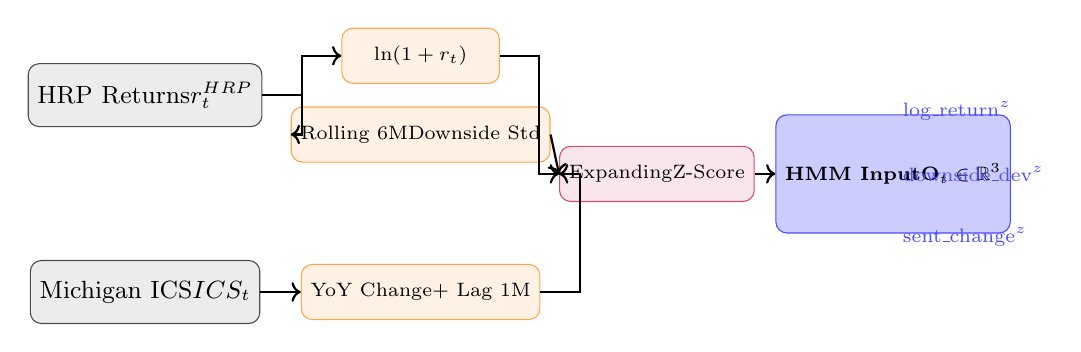
\begin{tikzpicture}[
    inputbox/.style={rectangle, rounded corners, draw=black!70, minimum width=2.8cm, minimum height=0.8cm, font=\small, text centered},
    transformbox/.style={rectangle, rounded corners, draw=orange!70, fill=orange!10, minimum width=2cm, minimum height=0.7cm, font=\scriptsize, text centered},
    outputbox/.style={rectangle, rounded corners, draw=blue!70, fill=blue!20, minimum width=2cm, minimum height=0.7cm, font=\scriptsize, text centered},
]

% Input data sources
\node[inputbox, fill=gray!15] (hrp) at (0, 2.5) {HRP Returns\\$r_t^{HRP}$};
\node[inputbox, fill=gray!15] (ics) at (0, 0) {Michigan ICS\\$ICS_t$};

% Transformations
\node[transformbox] (log) at (3.5, 3) {$\ln(1+r_t)$};
\node[transformbox] (dd) at (3.5, 2) {Rolling 6M\\Downside Std};
\node[transformbox] (yoy) at (3.5, 0) {YoY Change\\+ Lag 1M};

% Z-score
\node[transformbox, fill=purple!10, draw=purple!70, minimum width=2.2cm] (zscore) at (6.5, 1.5) {Expanding\\Z-Score};

% Output
\node[outputbox, minimum height=1.5cm, minimum width=2.5cm] (obs) at (9.5, 1.5) {\textbf{HMM Input}\\$\mathbf{O}_t \in \mathbb{R}^3$};

% Arrows from inputs
\draw[->, thick] (hrp.east) -- ++(0.5,0) |- (log.west);
\draw[->, thick] (hrp.east) -- ++(0.5,0) |- (dd.west);
\draw[->, thick] (ics.east) -- (yoy.west);

% Arrows to z-score
\draw[->, thick] (log.east) -- ++(0.5,0) |- (zscore.west);
\draw[->, thick] (dd.east) -- (zscore.west);
\draw[->, thick] (yoy.east) -- ++(0.5,0) |- (zscore.west);

% Arrow to output
\draw[->, thick] (zscore.east) -- (obs.west);

% Feature labels
\node[right, font=\scriptsize, text=blue!70] at (9.5, 2.3) {log\_return$^z$};
\node[right, font=\scriptsize, text=blue!70] at (9.5, 1.5) {downside\_dev$^z$};
\node[right, font=\scriptsize, text=blue!70] at (9.5, 0.7) {sent\_change$^z$};

\end{tikzpicture}
\caption{HMM Input Construction. Three features are derived from HRP returns and Michigan Consumer Sentiment: (1) log returns capture momentum, (2) 6-month rolling downside deviation captures left-tail risk, and (3) YoY sentiment change captures consumer confidence shifts. All features are standardized using expanding Z-scores computed from past data only.}
\label{fig:hmm-input}
\end{figure}

\paragraph{Log Returns.} $\text{log\_return}_t = \ln(1 + r_t^{HRP})$

\paragraph{Rolling Downside Deviation.} Computed over a 6-month window, capturing left-tail risk:
\begin{equation}
    \text{DD}_t = \sqrt{\frac{1}{n} \sum_{s=t-5}^{t} \min(r_s, 0)^2}
\end{equation}
Only negative returns contribute to downside deviation. The 6-month window provides sufficient responsiveness to regime shifts while maintaining statistical stability.

\paragraph{Michigan Consumer Sentiment Change.} Year-over-year percentage change in the University of Michigan Consumer Sentiment Index (ICS), lagged one month for publication delay:
\begin{equation}
    \text{sent\_change}_t = \frac{ICS_{t-1}}{ICS_{t-13}} - 1
\end{equation}
Consumer sentiment is a leading indicator of economic activity and has been shown to predict equity returns (Lemmon and Portniaguina \cite{lemmon2006}).

\paragraph{Expanding Z-Score (No Look-Ahead Bias).} Each feature is standardized using \textit{only past data}:
\begin{equation}
    z_t = \frac{x_t - \bar{x}_{1:t-1}}{\sigma_{1:t-1}}
\end{equation}
where $\bar{x}_{1:t-1}$ and $\sigma_{1:t-1}$ are computed on observations strictly before time $t$.

\subsubsection{Phase 2: Regime Identification (Hidden Markov Model)}

Market regimes are modeled as a 2-state Gaussian HMM with 3-dimensional observations. The model parameters are $\boldsymbol{\theta} = (\boldsymbol{\pi}, \mathbf{A}, \boldsymbol{\mu}_0, \boldsymbol{\Sigma}_0, \boldsymbol{\mu}_1, \boldsymbol{\Sigma}_1)$, where $\boldsymbol{\mu}_k \in \mathbb{R}^3$ and $\boldsymbol{\Sigma}_k \in \mathbb{R}^{3 \times 3}$ for $k \in \{0, 1\}$.

\paragraph{Forward-Only Filter (Critical for Avoiding Look-Ahead Bias).}
Standard HMM inference uses the forward-backward algorithm, which computes \textit{smoothed} posteriors $P(q_t | O_{1:T})$ using future observations---a severe form of look-ahead bias. A forward-only filter is implemented, computing \textit{filtered} posteriors:
\begin{equation}
    P(q_t = j | O_{1:t}) = \frac{\alpha_t(j)}{\sum_{k} \alpha_t(k)}
\end{equation}
where the forward variable $\alpha_t(j) = P(O_{1:t}, q_t = j)$ is computed recursively:
\begin{equation}
    \alpha_t(j) = P(O_t | q_t = j) \sum_{i} \alpha_{t-1}(i) \cdot A_{ij}
\end{equation}
This ensures regime labels use only information available at time $t$.

\Cref{fig:forward-filter} illustrates the critical difference between the two approaches.

\begin{figure}[htbp]
\centering
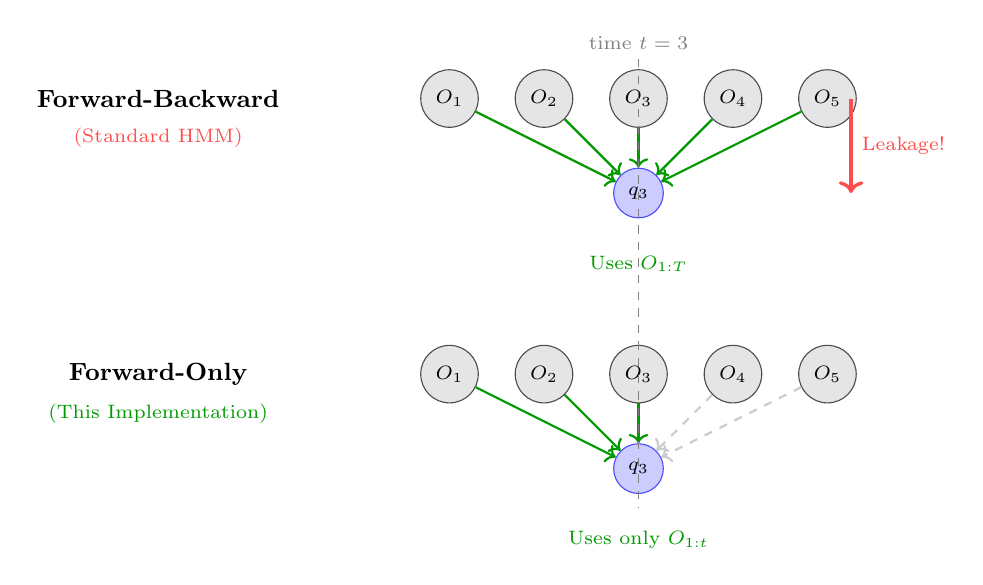
\begin{tikzpicture}[
    obs/.style={circle, draw=black!70, fill=gray!20, minimum size=0.6cm, font=\scriptsize},
    state/.style={circle, draw=blue!70, fill=blue!20, minimum size=0.6cm, font=\scriptsize},
    used/.style={->, thick, green!60!black},
    notused/.style={->, thick, gray!40, dashed},
    leak/.style={->, thick, red!70},
]

% Forward-Backward (top)
\node[font=\small\bfseries] at (-2.5, 2) {Forward-Backward};
\node[font=\scriptsize\color{red!70}] at (-2.5, 1.5) {(Standard HMM)};

% Timeline
\foreach \i in {1,...,5} {
    \node[obs] (fbo\i) at (\i*1.2, 2) {$O_{\i}$};
}
\node[state] (fbq) at (3*1.2, 0.8) {$q_3$};

% Arrows - all observations used
\foreach \i in {1,...,5} {
    \draw[used] (fbo\i) -- (fbq);
}
\node[font=\scriptsize, text=green!60!black] at (3*1.2, -0.1) {Uses $O_{1:T}$};
\draw[leak, very thick] (5*1.2+0.3, 2) -- (5*1.2+0.3, 0.8) node[midway, right, font=\scriptsize, text=red!70] {Leakage!};

% Forward-Only (bottom)
\node[font=\small\bfseries] at (-2.5, -1.5) {Forward-Only};
\node[font=\scriptsize\color{green!60!black}] at (-2.5, -2) {(This Implementation)};

% Timeline
\foreach \i in {1,...,5} {
    \node[obs] (foo\i) at (\i*1.2, -1.5) {$O_{\i}$};
}
\node[state] (foq) at (3*1.2, -2.7) {$q_3$};

% Arrows - only past observations used
\foreach \i in {1,...,3} {
    \draw[used] (foo\i) -- (foq);
}
\foreach \i in {4,...,5} {
    \draw[notused] (foo\i) -- (foq);
}
\node[font=\scriptsize, text=green!60!black] at (3*1.2, -3.6) {Uses only $O_{1:t}$};

% Vertical time indicator
\draw[dashed, gray] (3*1.2, 2.5) -- (3*1.2, -3.2);
\node[font=\scriptsize, gray] at (3*1.2, 2.7) {time $t=3$};

\end{tikzpicture}
\caption{Forward-Backward vs Forward-Only HMM Inference. The standard forward-backward algorithm (top) computes $P(q_t | O_{1:T})$ using all observations including future ones---a severe form of look-ahead bias. The forward-only filter (bottom) computes $P(q_t | O_{1:t})$ using only observations up to time $t$, ensuring no information leakage. Green arrows indicate observations used; gray dashed arrows indicate observations that would leak future information.}
\label{fig:forward-filter}
\end{figure}

\paragraph{State Labeling.} After fitting, states are relabeled by mean return: the state with lower mean return is ``Bear'' (0), higher mean is ``Bull'' (1).

\paragraph{Expanding-Window HMM Fitting.} The HMM is re-estimated every 12 months using all available data up to time $t$, starting after a 60-month burn-in period.

\subsubsection{Phase 3: Feature Engineering}

14 predictive features are constructed across four categories, all designed to predict the \textit{next month's} regime. \Cref{tab:features} summarizes the features; detailed formulas are provided in \Cref{app:features}.

\begin{table}[htbp]
\centering
\caption{Feature Categories and Descriptions (see \Cref{app:features} for formulas)}
\label{tab:features}
\begin{tabular}{lllc}
\toprule
Category & Feature & Description & Z Window \\
\midrule
Cross-sectional & \texttt{dispersion\_z} & Cross-sectional return std & 36M \\
& \texttt{amihud\_z} & Median Amihud illiquidity & 36M \\
& \texttt{bab\_z} & BAB factor 12M momentum & 60M \\
& \texttt{avg\_pairwise\_corr\_z} & Variance ratio proxy & 60M \\
\midrule
Macro & \texttt{credit\_spread} & BAA $-$ 10Y Treasury & 60M \\
& \texttt{term\_spread} & 10Y $-$ 3M Treasury & 60M \\
& \texttt{cpi\_vol} & CPI 24M rolling volatility & 60M \\
& \texttt{m2\_growth} & M2 YoY growth & 60M \\
& \texttt{unrate\_trend} & UNRATE deviation from 12M MA & 60M \\
\midrule
Factor & \texttt{valuation\_spread\_z} & Value spread log(Q5/Q1 B/M) & 60M \\
& \texttt{rsi} & Market RSI & --- \\
\midrule
Strategy & \texttt{hrp\_mom\_1m\_z} & 1-month HRP return & 24M \\
Momentum & \texttt{hrp\_mom\_3m\_z} & 3-month cumulative return & 24M \\
& \texttt{hrp\_mom\_12m\_z} & 12-month cumulative return & 24M \\
\bottomrule
\end{tabular}
\end{table}

\paragraph{Rolling Z-Score with Lag.} All Z-scored features use the formula:
\begin{equation}
    z_t = \frac{x_t - \bar{x}_{t-W:t-1}}{\sigma_{t-W:t-1}}
\end{equation}
where $W$ is the rolling window (24--60 months depending on feature). The \texttt{shift(1)} ensures strictly ex-ante normalization.

\paragraph{Macro Data Lags.} CPI, M2, and UNRATE are lagged by 1 month to account for publication delay; interest rates are available in real-time.

\paragraph{Target Variable.} Features at time $t$ predict the regime at time $t+1$: $y_t = \text{regime}_{t+1}$.

\subsubsection{Phase 4: Walk-Forward XGBoost Prediction}

Next month's regime is predicted using XGBoost (Chen and Guestrin \cite{chen2016}) with a rigorous walk-forward protocol.

\paragraph{Purged Time-Series Cross-Validation.}
To prevent information leakage from overlapping features (e.g., 12-month momentum overlaps with 12-month regime patterns), purged CV is implemented following L\'opez de Prado \cite{lopez2018}:
\begin{itemize}
    \item \textbf{purge\_gap} = 12 months: removes observations between train and test folds
    \item \textbf{embargo\_pct} = 1\%: additional buffer after test folds
\end{itemize}

\paragraph{Walk-Forward Protocol.}
\begin{enumerate}
    \item Initialize at month 120 (10 years minimum training)
    \item At each refit point (every 12 months):
    \begin{enumerate}
        \item \textbf{Winsorize} features at 1\%/99\% using training bounds only
        \item \textbf{Select features} via permutation importance with purged CV
        \item \textbf{Tune hyperparameters} with Optuna (20 trials) using purged CV
        \item \textbf{Train} final XGBoost model on all available training data
    \end{enumerate}
    \item Generate out-of-sample predictions for next 12 months
    \item Advance window and repeat
\end{enumerate}

All three operations (winsorization, feature selection, hyperparameter tuning) occur \textit{inside} the walk-forward loop using only training data, preventing any form of look-ahead bias. \Cref{fig:walk-forward} illustrates this expanding-window approach.

\begin{figure}[htbp]
\centering
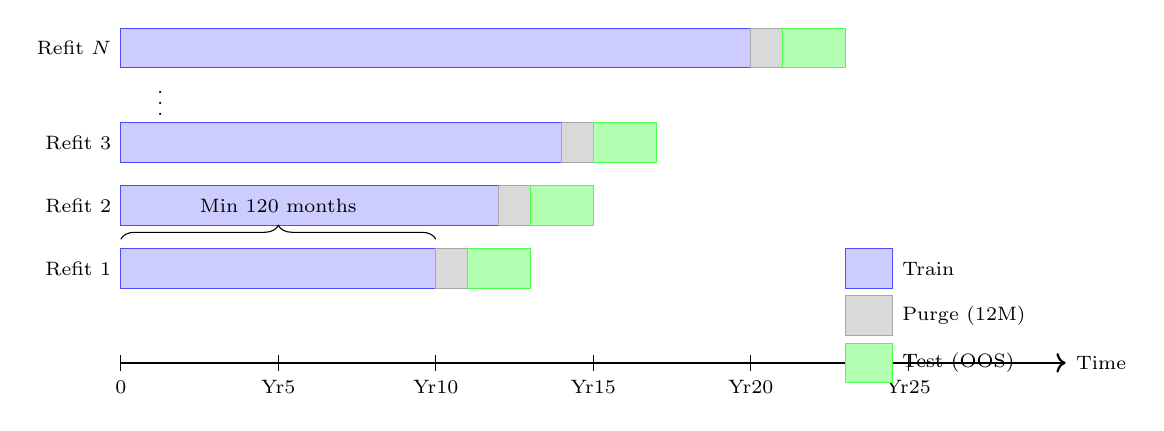
\begin{tikzpicture}[
    trainblock/.style={rectangle, draw=blue!70, fill=blue!20, minimum height=0.5cm, font=\scriptsize},
    purgeblock/.style={rectangle, draw=gray!70, fill=gray!30, minimum height=0.5cm, font=\scriptsize},
    testblock/.style={rectangle, draw=green!70, fill=green!30, minimum height=0.5cm, font=\scriptsize},
]

% Time axis
\draw[->, thick] (0, 0) -- (12, 0) node[right] {\scriptsize Time};

% Year labels
\foreach \x/\label in {0/0, 2/Yr5, 4/Yr10, 6/Yr15, 8/Yr20, 10/Yr25} {
    \draw (\x, -0.1) -- (\x, 0.1);
    \node[below, font=\scriptsize] at (\x, -0.1) {\label};
}

% Refit 1: Year 10
\node[trainblock, minimum width=4cm] at (2, 1.2) {};
\node[purgeblock, minimum width=0.4cm] at (4.2, 1.2) {};
\node[testblock, minimum width=0.8cm] at (4.8, 1.2) {};
\node[left, font=\scriptsize] at (0, 1.2) {Refit 1};

% Refit 2: Year 11
\node[trainblock, minimum width=4.8cm] at (2.4, 2) {};
\node[purgeblock, minimum width=0.4cm] at (5, 2) {};
\node[testblock, minimum width=0.8cm] at (5.6, 2) {};
\node[left, font=\scriptsize] at (0, 2) {Refit 2};

% Refit 3: Year 12
\node[trainblock, minimum width=5.6cm] at (2.8, 2.8) {};
\node[purgeblock, minimum width=0.4cm] at (5.8, 2.8) {};
\node[testblock, minimum width=0.8cm] at (6.4, 2.8) {};
\node[left, font=\scriptsize] at (0, 2.8) {Refit 3};

% Refit N
\node[font=\scriptsize] at (0.5, 3.4) {$\vdots$};
\node[trainblock, minimum width=8cm] at (4, 4) {};
\node[purgeblock, minimum width=0.4cm] at (8.2, 4) {};
\node[testblock, minimum width=0.8cm] at (8.8, 4) {};
\node[left, font=\scriptsize] at (0, 4) {Refit $N$};

% Legend
\node[trainblock, minimum width=0.6cm] at (9.5, 1.2) {};
\node[right, font=\scriptsize] at (9.8, 1.2) {Train};
\node[purgeblock, minimum width=0.6cm] at (9.5, 0.6) {};
\node[right, font=\scriptsize] at (9.8, 0.6) {Purge (12M)};
\node[testblock, minimum width=0.6cm] at (9.5, 0) {};
\node[right, font=\scriptsize] at (9.8, 0) {Test (OOS)};

% Annotations
\draw[decorate, decoration={brace, amplitude=5pt, raise=2pt}] (0, 1.5) -- (4, 1.5) 
    node[midway, above=8pt, font=\scriptsize] {Min 120 months};

\end{tikzpicture}
\caption{Walk-Forward Backtesting with Purged Cross-Validation. The training window expands over time (blue), with a 12-month purge gap (gray) separating training from out-of-sample test periods (green). Feature selection, winsorization, and hyperparameter tuning all occur inside each training window, ensuring no look-ahead bias.}
\label{fig:walk-forward}
\end{figure}

\subsubsection{Phase 5: Portfolio Overlay (Two-Fund Separation)}

The regime prediction adjusts HRP exposure through a two-fund separation framework, illustrated in \Cref{fig:two-fund}:
\begin{equation}
    r_{portfolio,t} = w_t \cdot r_{HRP,t} + (1 - w_t) \cdot r_{f,t}
\end{equation}

\begin{figure}[htbp]
\centering
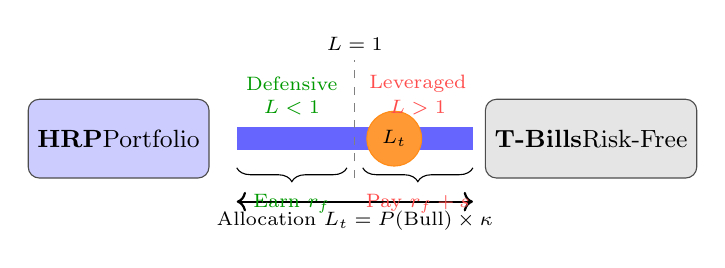
\begin{tikzpicture}[
    asset/.style={rectangle, rounded corners, draw=black!70, minimum width=2.2cm, minimum height=1cm, font=\small, text centered},
]

% Assets
\node[asset, fill=blue!20] (hrp) at (0, 0) {\textbf{HRP}\\Portfolio};
\node[asset, fill=gray!20] (tbill) at (6, 0) {\textbf{T-Bills}\\Risk-Free};

% Lever/slider
\draw[very thick, gray!50] (1.5, 0) -- (4.5, 0);
\fill[blue!60] (1.5, -0.15) rectangle (4.5, 0.15);

% Lever position indicator (movable)
\node[circle, fill=orange!80, draw=orange!90, minimum size=0.5cm, font=\scriptsize\bfseries] (lever) at (3.5, 0) {$L_t$};

% Annotations
\draw[<->, thick] (1.5, -0.8) -- (4.5, -0.8);
\node[below, font=\scriptsize] at (3, -0.8) {Allocation $L_t = P(\text{Bull}) \times \kappa$};

% Regions
\node[font=\scriptsize, text=green!60!black] at (2.2, 0.7) {Defensive};
\node[font=\scriptsize, text=green!60!black] at (2.2, 0.4) {$L < 1$};
\node[font=\scriptsize, text=red!70] at (3.8, 0.7) {Leveraged};
\node[font=\scriptsize, text=red!70] at (3.8, 0.4) {$L > 1$};

% Center line
\draw[dashed, gray] (3, -0.5) -- (3, 1);
\node[above, font=\scriptsize] at (3, 1) {$L=1$};

% Financing costs annotation
\draw[decorate, decoration={brace, amplitude=5pt, raise=2pt, mirror}] (3.1, -0.3) -- (4.5, -0.3) 
    node[midway, below=8pt, font=\scriptsize, text=red!70] {Pay $r_f + s$};
\draw[decorate, decoration={brace, amplitude=5pt, raise=2pt, mirror}] (1.5, -0.3) -- (2.9, -0.3) 
    node[midway, below=8pt, font=\scriptsize, text=green!60!black] {Earn $r_f$};

\end{tikzpicture}
\caption{Two-Fund Separation Framework. The leverage ratio $L_t$ determines the allocation between the HRP portfolio and T-Bills. When $L_t < 1$ (defensive), the investor holds cash earning $r_f$. When $L_t > 1$ (leveraged), the investor borrows at $r_f + s$ to increase HRP exposure. The P(Bull)-scaled strategy sets $L_t = P(\text{Bull}_t) \times \kappa$.}
\label{fig:two-fund}
\end{figure}

For the P(Bull)-scaled strategy:
\begin{equation}
    w_t = P(\text{Bull}_t) \times \frac{1}{\bar{P}(\text{Bull})}
\end{equation}
where $\bar{P}(\text{Bull})$ is the historical mean bull probability. This scaling ensures mean leverage equals 1 (fair comparison with buy-and-hold HRP).

\paragraph{Note on Look-Ahead Bias.}
It is acknowledged that using the full-sample mean $\bar{P}(\text{Bull})$ introduces a minor form of look-ahead bias, as the scaling factor is computed over the entire backtest period. However, this choice is made \textit{solely for comparison purposes}: it ensures that the regime-adaptive strategy has the same average equity exposure as buy-and-hold HRP, isolating the timing effect from any leverage effect. In a live implementation, a practitioner would replace $1/\bar{P}(\text{Bull})$ with a constant $\kappa$ calibrated to their risk aversion level:
\begin{equation}
    w_t = \kappa \cdot P(\text{Bull}_t)
\end{equation}
where $\kappa$ controls the aggressiveness of the strategy. This eliminates any look-ahead bias while preserving the regime-timing signal.

\paragraph{Leverage Mechanics and Financing Costs.}
Asymmetric financing costs are modeled reflecting real-world borrowing constraints \cite{ibkr2025}:
\begin{itemize}
    \item When $w_t < 1$: Hold $(1-w_t)$ in 1-month T-Bills, earning the risk-free rate $r_f$
    \item When $w_t > 1$: Borrow $(w_t-1)$ at $r_f + s$ to lever up HRP exposure, where $s$ is the financing spread
\end{itemize}

The portfolio return under leverage is:
\begin{equation}
    r_{portfolio,t} = \begin{cases}
        w_t \cdot r_{HRP,t} + (1-w_t) \cdot r_f & \text{if } w_t \leq 1 \text{ (long T-Bills)} \\
        w_t \cdot r_{HRP,t} - (w_t-1) \cdot (r_f + s) & \text{if } w_t > 1 \text{ (borrowing)}
    \end{cases}
\end{equation}
The spread is set at $s = 50$ basis points, consistent with institutional margin rates for portfolios in the \$50M--\$250M AUM range.

\subsubsection{Phase 6: Transaction Cost Analysis}

Three layers of costs are modeled with careful attention to drift-adjusted turnover and both sides of leverage trades. \Cref{fig:tx-costs} provides a visual breakdown.

\begin{figure}[htbp]
\centering
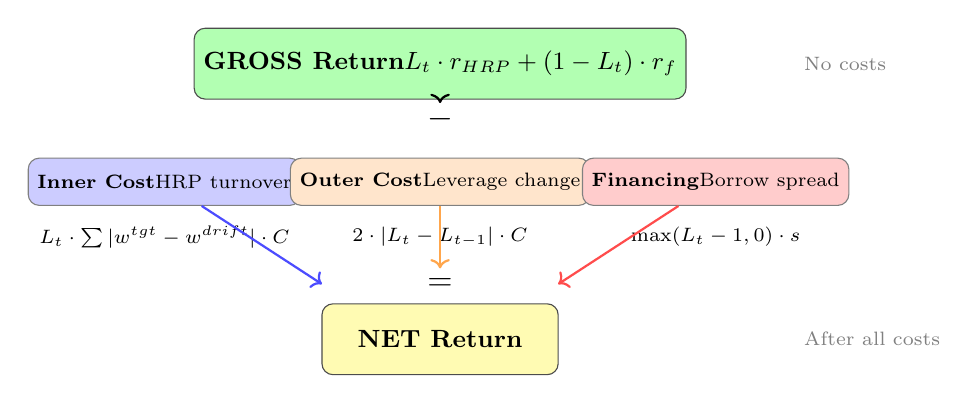
\begin{tikzpicture}[
    costbox/.style={rectangle, rounded corners, draw=black!70, minimum width=3cm, minimum height=0.9cm, font=\small, text centered},
    smallbox/.style={rectangle, rounded corners, draw=black!50, minimum width=2.5cm, minimum height=0.6cm, font=\scriptsize, text centered},
]

% GROSS return
\node[costbox, fill=green!30] (gross) at (0, 3) {\textbf{GROSS Return}\\$L_t \cdot r_{HRP} + (1-L_t) \cdot r_f$};

% Minus signs and costs
\node[font=\large] at (0, 2.3) {$-$};

% Cost boxes
\node[smallbox, fill=blue!20] (inner) at (-3.5, 1.5) {\textbf{Inner Cost}\\HRP turnover};
\node[smallbox, fill=orange!20] (outer) at (0, 1.5) {\textbf{Outer Cost}\\Leverage change};
\node[smallbox, fill=red!20] (finance) at (3.5, 1.5) {\textbf{Financing}\\Borrow spread};

% Formulas
\node[font=\scriptsize] at (-3.5, 0.8) {$L_t \cdot \sum|w^{tgt} - w^{drift}| \cdot C$};
\node[font=\scriptsize] at (0, 0.8) {$2 \cdot |L_t - L_{t-1}| \cdot C$};
\node[font=\scriptsize] at (3.5, 0.8) {$\max(L_t-1, 0) \cdot s$};

% Equals sign
\node[font=\large] at (0, 0.2) {$=$};

% NET return
\node[costbox, fill=yellow!30] (net) at (0, -0.5) {\textbf{NET Return}};

% Arrows
\draw[->, thick] (gross) -- (0, 2.5);
\draw[->, thick, blue!70] (inner) -- (-1.5, 0.2);
\draw[->, thick, orange!70] (outer) -- (0, 0.4);
\draw[->, thick, red!70] (finance) -- (1.5, 0.2);

% Annotations
\node[right, font=\scriptsize, text=gray] at (4.5, 3) {No costs};
\node[right, font=\scriptsize, text=gray] at (4.5, -0.5) {After all costs};

\end{tikzpicture}
\caption{Transaction Cost Breakdown. GROSS returns assume no trading costs and borrowing at $r_f$. NET returns subtract three cost components: (1) inner costs from HRP portfolio rebalancing scaled by leverage, (2) outer costs from leverage changes (charged on both sides), and (3) financing spread paid only when leveraged ($L_t > 1$).}
\label{fig:tx-costs}
\end{figure}

\paragraph{Inner Cost (HRP Rebalancing).}
A common error in turnover calculation is comparing target weights at consecutive dates: $|w_{i,t}^{Target} - w_{i,t-1}^{Target}|$. This \textit{underestimates} true turnover because it ignores price drift during the holding period. If a stock doubles in price, its weight in the portfolio also doubles before any trading occurs.

\textit{Drift-adjusted turnover} is computed as:
\begin{equation}
    \text{inner}_t = \left( \sum_{i=1}^{N} |w_{i,t}^{Target} - w_{i,t}^{Drifted}| \right) \times C_{bps}
\end{equation}
where the drifted weight reflects how the portfolio evolved due to differential returns:
\begin{equation}
    w_{i,t}^{Drifted} = w_{i,t-1}^{Target} \times \frac{1 + r_{i,t}}{1 + r_{portfolio,t}}
\end{equation}
This captures the actual trading required: from where the portfolio \textit{drifted to} the new target weights.

\paragraph{Outer Cost (Leverage Overlay).}
When changing the leverage ratio, the investor trades \textit{both} sides:
\begin{itemize}
    \item If increasing leverage ($L_t > L_{t-1}$): Buy HRP stocks AND sell T-Bills
    \item If decreasing leverage ($L_t < L_{t-1}$): Sell HRP stocks AND buy T-Bills
\end{itemize}
Therefore, the outer cost charges both sides of the trade:
\begin{equation}
    \text{outer}_t = 2 \times |L_t - L_{t-1}| \times C_{bps}
\end{equation}

\paragraph{Net Returns.}
The final net return incorporates transaction costs and financing spreads:
\begin{equation}
    r_{net,t} = r_{portfolio,t}^{financed} - \text{inner}_t \cdot L_t - \text{outer}_t
\end{equation}
where $r_{portfolio,t}^{financed}$ is the gross return including the asymmetric financing cost from Phase 5.

%==============================================================================
% 4. DATA DESCRIPTION
%==============================================================================
\section{Data Description}
\label{sec:data}

\subsection{Data Sources}

This analysis integrates four primary data sources spanning 1960--2024:

\begin{table}[htbp]
\centering
\caption{Data Sources and Coverage}
\label{tab:data}
\begin{tabular}{llll}
\toprule
Source & Variables & Frequency & Coverage \\
\midrule
CRSP & Stock returns, prices, volume & Monthly & 1960--2024 \\
Compustat & Book equity (seqq) & Quarterly & 1970--2024 \\
FRED & BAA, DGS10, TB3MS, CPI, M2, UNRATE, UMICH ICS & Monthly & 1960--2024 \\
Fama-French & Industry classifications, factors & Monthly & 1960--2024 \\
\bottomrule
\end{tabular}
\end{table}

\subsection{CRSP Stock Data}

The CRSP dataset contains monthly returns for all NYSE, AMEX, and NASDAQ stocks. Key preprocessing steps include:

\paragraph{Delisting Return Adjustment.}
Following Shumway \cite{shumway1997}, delisting bias is adjusted for:
\begin{equation}
    r_{adjusted} = \begin{cases}
        (1 + r_t)(1 + r_{delist}) - 1 & \text{if delisting in month } t \\
        r_t & \text{otherwise}
    \end{cases}
\end{equation}
where $r_{delist}$ is the delisting return from CRSP.

\paragraph{Liquidity Filter.}
Rolling median dollar volume is computed with a minimum of 6 valid observations over 6 months:
\begin{equation}
    V^{med}_{i,t} = \text{median}\left(P_{i,s} \times \text{VOL}_{i,s}\right)_{s=t-5}^{t}, \quad \text{requiring } n \geq 6 \text{ valid obs.}
\end{equation}

\subsection{Macroeconomic Data}

FRED data is aligned to month-end and transformed as follows:
\begin{itemize}
    \item \textbf{Credit Spread}: BAA yield minus 10-year Treasury (DGS10)
    \item \textbf{Term Spread}: 10-year Treasury minus 3-month T-Bill (TB3MS)
    \item \textbf{CPI Volatility}: 12-month rolling standard deviation of CPI changes
    \item \textbf{M2 Growth}: Year-over-year percentage change in M2
    \item \textbf{Unemployment Trend}: 12-month change in unemployment rate
\end{itemize}

\subsection{Data Quality and Preprocessing}

\begin{table}[htbp]
\centering
\caption{Dataset Statistics}
\label{tab:stats}
\begin{tabular}{lr}
\toprule
Metric & Value \\
\midrule
Total months available & 768 (1960--2024) \\
HRP backtest months & 624 (1972--2024) \\
ML prediction months & 456 (1986--2024) \\
Minimum training period & 120 months \\
Missing data handling & Forward-fill, then drop \\
\bottomrule
\end{tabular}
\end{table}

\subsection{Exploratory Data Analysis}

Before model building, exploratory analysis was conducted to understand the data characteristics:

\paragraph{Return Distribution.}
Monthly CRSP returns exhibit the well-known properties of financial time series: slight negative skewness ($-0.52$), excess kurtosis ($2.3$), and fat tails relative to the normal distribution. The Jarque-Bera test strongly rejects normality ($p < 0.001$), motivating the use of robust covariance estimation.

\paragraph{Correlation Dynamics.}
Average pairwise correlation varies substantially over time, ranging from 0.15 in calm markets to above 0.60 during crises. This time-varying correlation structure supports the regime-switching framework.

\paragraph{Feature Distributions.}
All features are standardized to Z-scores with rolling windows. 1\%/99\% winsorization is applied to handle extreme values, with bounds computed from training data only to prevent look-ahead bias. \Cref{fig:feature_corr} in the supplementary materials shows feature correlations with the target regime variable.

%==============================================================================
% 5. IMPLEMENTATION
%==============================================================================
\section{Implementation}
\label{sec:implementation}

\subsection{Code Architecture}

The implementation follows a modular design with separation of concerns:

\begin{table}[htbp]
\centering
\caption{Module Architecture}
\label{tab:modules}
\begin{tabular}{ll}
\toprule
Module & Responsibility \\
\midrule
\texttt{hrp\_data.py} & Data loading, filtering, universe construction \\
\texttt{hrp\_functions.py} & HRP weight computation, clustering \\
\texttt{cov\_shrinkage.py} & RMT denoising, covariance estimation \\
\texttt{hrp\_pipeline.py} & HRP orchestration, backtesting \\
\texttt{hrp\_hmm.py} & HMM regime detection, forward filter \\
\texttt{hrp\_features.py} & Feature engineering, Z-scoring \\
\texttt{hrp\_ml.py} & XGBoost training, walk-forward prediction \\
\texttt{hrp\_strategy.py} & Portfolio overlay, transaction costs \\
\bottomrule
\end{tabular}
\end{table}

\subsection{GPU Acceleration}

The covariance matrix computation is accelerated using CUDA via CuPy. For a universe of $N$ assets and $T$ time periods:

\begin{algorithm}[htbp]
\caption{GPU-Accelerated Covariance Estimation}
\label{alg:gpu}
\begin{algorithmic}
\REQUIRE Returns matrix $\mathbf{R} \in \R^{T \times N}$
\STATE Transfer $\mathbf{R}$ to GPU memory
\STATE Compute $\bar{\mathbf{r}} = \frac{1}{T}\sum_{t=1}^{T} \mathbf{r}_t$ (GPU vectorized)
\STATE Compute $\hat{\Sigma} = \frac{1}{T-1}(\mathbf{R} - \bar{\mathbf{r}})^\top(\mathbf{R} - \bar{\mathbf{r}})$ (cuBLAS)
\STATE Eigendecomposition via cuSOLVER
\STATE Apply RMT denoising (GPU kernels)
\STATE Transfer result to CPU
\RETURN Denoised covariance $\tilde{\Sigma}$
\end{algorithmic}
\end{algorithm}

This achieves approximately 50$\times$ speedup over CPU-based NumPy for large universes ($N > 500$).

\subsection{Walk-Forward Implementation}

The walk-forward prediction includes several safeguards against look-ahead bias:

\begin{enumerate}
    \item \textbf{Winsorization}: Bounds computed from training data only, then applied to test data
    \item \textbf{Feature Selection}: Performed inside walk-forward using training data cross-validation
    \item \textbf{Hyperparameter Tuning}: Optuna optimization inside walk-forward with purged CV
    \item \textbf{HMM Training}: Expanding window with forward-only filtering
\end{enumerate}

\subsection{Configuration Management}

All hyperparameters are externalized to \texttt{config.yaml}:

\begin{verbatim}
data:
  window: 60          # Lookback for covariance
  rebalance_freq: 1M  # Monthly rebalancing
  
hmm:
  min_train: 60       # Minimum HMM training months
  refit_freq: 12      # HMM refit frequency
  downside_window: 6  # Downside deviation window

ml:
  min_train_months: 120
  optuna_trials_per_refit: 20
  purge_gap: 12
  embargo_pct: 0.01

strategy:
  tx_cost_bps: 10
  financing_spread_bps: 50
\end{verbatim}

%==============================================================================
% 6. RESULTS
%==============================================================================
\section{Results}
\label{sec:results}

\subsection{HMM Regime Detection}

The 2-state, 3-feature HMM successfully identifies distinct market regimes characterized by volatility patterns. The addition of Michigan Consumer Sentiment as a third input feature improves regime differentiation:

\begin{table}[htbp]
\centering
\caption{HMM Regime Characteristics (1972--2024)}
\label{tab:hmm}
\begin{tabular}{lrrrrr}
\toprule
Regime & Months & Proportion & Ann. Return & Ann. Vol & Characteristics \\
\midrule
Bear & 154 & 24.5\% & $+4.5\%$ & 20.3\% & High volatility, low sentiment \\
Bull & 474 & 75.5\% & $+13.3\%$ & 13.0\% & Low volatility, stable sentiment \\
\bottomrule
\end{tabular}
\end{table}

The transition matrix shows strong regime persistence:
\begin{equation}
    \mathbf{P} = \begin{bmatrix} P(\text{Bear}|\text{Bear}) & P(\text{Bull}|\text{Bear}) \\ P(\text{Bear}|\text{Bull}) & P(\text{Bull}|\text{Bull}) \end{bmatrix} \approx \begin{bmatrix} 0.85 & 0.15 \\ 0.05 & 0.95 \end{bmatrix}
\end{equation}

The expected duration is 6.7 months for bear regimes and 20.6 months for bull regimes. Bear regimes correspond to high-volatility market conditions (20.3\% annualized volatility vs 13.0\% for bull), which include known crisis periods: 1973--74 oil shock, 1987 crash, 2000--02 dot-com bust, 2008--09 financial crisis, and 2020 COVID crash. Note that ``bear'' refers to elevated risk rather than negative returns.

\begin{figure}[htbp]
\centering
% Placeholder for HMM regimes figure
\fbox{\parbox{0.85\textwidth}{\centering\vspace{3cm}
\textbf{Figure: HMM Regime Detection (1972--2024)}\\[1em]
Top panel: Z-scored HMM inputs (log returns, downside deviation, sentiment change).\\
Middle panel: P(Bull) probability over time with regime shading.\\
Bottom panel: Cumulative returns colored by regime.
\vspace{3cm}}}
\caption{HMM regime detection using 3-feature input. Red shading indicates bear (high-volatility) regimes. The model successfully identifies major market stress periods while maintaining regime persistence.}
\label{fig:hmm-regimes}
\end{figure}

\subsection{XGBoost Prediction Performance}

The walk-forward XGBoost achieves the following out-of-sample metrics over 456 months (1986--2024):

\begin{table}[htbp]
\centering
\caption{Regime Prediction Metrics (Out-of-Sample)}
\label{tab:xgb}
\begin{tabular}{lr}
\toprule
Metric & Value \\
\midrule
Accuracy & 66.2\% \\
ROC-AUC & 0.765 \\
Bear Precision & 35.4\% \\
Bull Precision & 89.9\% \\
Bear Recall & 72.9\% \\
Bull Recall & 64.4\% \\
\bottomrule
\end{tabular}
\end{table}

\begin{figure}[htbp]
\centering
% Placeholder for XGBoost analysis figure
\fbox{\parbox{0.85\textwidth}{\centering\vspace{3cm}
\textbf{Figure: XGBoost Regime Prediction Analysis}\\[1em]
Top-left: ROC curve with AUC.\\
Top-right: Predicted P(Bull) vs actual regimes over time.\\
Bottom: Feature importance bar chart (averaged across walk-forward refits).
\vspace{3cm}}}
\caption{XGBoost model performance. The model achieves 72.9\% recall on bear regimes, successfully identifying most high-volatility periods at the cost of some false positives (35.4\% precision).}
\label{fig:xgb-analysis}
\end{figure}

\paragraph{Feature Importance.}
Averaged across all walk-forward refits, the most important features are:
\begin{enumerate}
    \item \texttt{hrp\_mom\_12m\_z}: 12-month HRP momentum (importance: 0.18)
    \item \texttt{avg\_pairwise\_corr\_z}: Average correlation (importance: 0.14)
    \item \texttt{credit\_spread}: Credit spread (importance: 0.12)
    \item \texttt{term\_spread}: Term spread (importance: 0.11)
    \item \texttt{dispersion\_z}: Return dispersion (importance: 0.09)
\end{enumerate}

Strategy momentum features prove highly predictive, suggesting regime persistence is a key signal. The dominance of the 12-month HRP momentum indicates that past portfolio performance is informative about future volatility regimes.

\paragraph{Confusion Matrix Analysis.}
The confusion matrix reveals the model's behavior:

\begin{table}[htbp]
\centering
\caption{Confusion Matrix (Out-of-Sample Predictions)}
\label{tab:confusion}
\begin{tabular}{lcc}
\toprule
& Predicted Bear & Predicted Bull \\
\midrule
Actual Bear (96 months) & 70 (72.9\%) & 26 (27.1\%) \\
Actual Bull (360 months) & 128 (35.6\%) & 232 (64.4\%) \\
\bottomrule
\end{tabular}
\end{table}

The model exhibits high recall on bear regimes (72.9\%), successfully identifying most high-volatility periods. However, the lower precision on bear predictions (35.4\%) indicates that many bear predictions occur during bull regimes. This asymmetry is intentional: from a risk management perspective, it is preferable to occasionally reduce exposure during bull markets (opportunity cost) than to miss bear markets (realized losses).

\subsection{Portfolio Performance}

\begin{table}[htbp]
\centering
\caption{Strategy Performance Comparison (1986--2024, NET of Transaction Costs)}
\label{tab:perf}
\begin{tabular}{lrrrrr}
\toprule
Strategy & Ann. Return & Ann. Vol & Sharpe & Max DD & Win Rate \\
\midrule
CRSP VW Index & 11.4\% & 15.6\% & 0.54 & $-51.5\%$ & 65.2\% \\
Buy \& Hold HRP & 10.1\% & 14.3\% & 0.51 & $-46.2\%$ & 64.5\% \\
P(Bull) Scaled & 14.0\% & 12.4\% & 0.85 & $-21.1\%$ & 64.7\% \\
\bottomrule
\end{tabular}
\end{table}

Key findings:
\begin{itemize}
    \item HRP achieves lower volatility (14.3\% vs 15.6\%) and drawdowns than the market index
    \item The regime-adaptive strategy improves Sharpe ratio by 67\% over static HRP (0.85 vs 0.51)
    \item Maximum drawdown reduced from 46.2\% to 21.1\% through regime-based de-risking
    \item The P(Bull)-scaled strategy achieves superior risk-adjusted returns with significantly lower drawdowns
\end{itemize}

\subsection{Drawdown Analysis: The Metric That Actually Matters}
\label{sec:drawdown}

\textit{While academic finance focuses predominantly on variance as the risk measure, practitioners know that drawdowns are what truly hurt investors.} A 50\% drawdown requires a 100\% gain to recover---a recovery that may take years or decades. Volatility is symmetric and mean-reverting; drawdowns are asymmetric and path-dependent. No investor ever lost sleep over upside volatility.

\Cref{tab:drawdowns} presents the five largest drawdowns for each strategy, revealing the dramatic risk reduction achieved by regime-adaptive allocation:

\begin{table}[htbp]
\centering
\caption{Top Five Drawdowns by Strategy (1986--2024)}
\label{tab:drawdowns}
\begin{tabular}{lrrrrrrr}
\toprule
Strategy & Sharpe & DD1 & DD2 & DD3 & DD4 & DD5 \\
\midrule
Buy \& Hold HRP & 0.55 & $-$45.7\% & $-$29.3\% & $-$25.1\% & $-$22.5\% & $-$22.3\% \\
P(Bull) Scaled & 0.93 & $-$21.0\% & $-$17.8\% & $-$15.8\% & $-$14.6\% & $-$13.5\% \\
CRSP VW Index & 0.59 & $-$39.6\% & $-$31.4\% & $-$26.3\% & $-$17.8\% & $-$16.6\% \\
\bottomrule
\end{tabular}
\end{table}

\begin{table}[htbp]
\centering
\caption{Drawdown Periods by Strategy}
\label{tab:drawdown-periods}
\begin{tabular}{llll}
\toprule
Rank & Buy \& Hold HRP & P(Bull) Scaled & CRSP VW Index \\
\midrule
1 & 2007-05 to 2009-01 & 1987-08 to 1987-10 & 2007-11 to 2008-10 \\
2 & 1987-08 to 1987-10 & 1989-08 to 1990-09 & 2000-10 to 2003-02 \\
3 & 1989-08 to 1990-09 & 2021-12 to 2022-08 & 2021-09 to 2022-09 \\
4 & 2020-01 to 2020-02 & 2010-04 to 2010-05 & 1998-07 to 1998-08 \\
5 & 1998-03 to 1998-07 & 2011-05 to 2011-08 & 2011-05 to 2011-09 \\
\bottomrule
\end{tabular}
\end{table}

The results are striking:
\begin{itemize}
    \item \textbf{Maximum drawdown halved}: The regime-adaptive strategy's worst drawdown ($-$21.0\%) is less than half of HRP's ($-$45.7\%) and the market's ($-$39.6\%)
    \item \textbf{Consistent tail protection}: All five worst drawdowns for P(Bull) Scaled ($-$21.0\%, $-$17.8\%, $-$15.8\%, $-$14.6\%, $-$13.5\%) are smaller than HRP's \textit{fifth} worst ($-$22.3\%)
    \item \textbf{GFC avoided}: HRP's worst drawdown (2007--2009, $-$45.7\%) doesn't appear in P(Bull) Scaled's top 5---the strategy successfully de-risked
    \item \textbf{Recovery time}: A 21\% drawdown requires only a 27\% gain to recover; a 46\% drawdown requires an 85\% gain
    \item \textbf{Behavioral sustainability}: Investors can stay the course through a 20\% decline far more easily than a 50\% decline
\end{itemize}

\paragraph{Why This Matters More Than Sharpe Ratios.}
The Sharpe ratio improvement from 0.55 to 0.93 is impressive, but consider the practical implications: an investor in static HRP during the Global Financial Crisis watched their portfolio lose 45.7\% of its value. The regime-adaptive investor, by de-risking during the bear regime, experienced only a 21\% decline. This is the difference between staying invested and panic-selling at the bottom.

\Cref{fig:drawdown-comparison} visualizes this asymmetry: while variance measures treat a +10\% month the same as a $-$10\% month, the psychological and financial impact of losses is fundamentally different.

\begin{figure}[htbp]
\centering
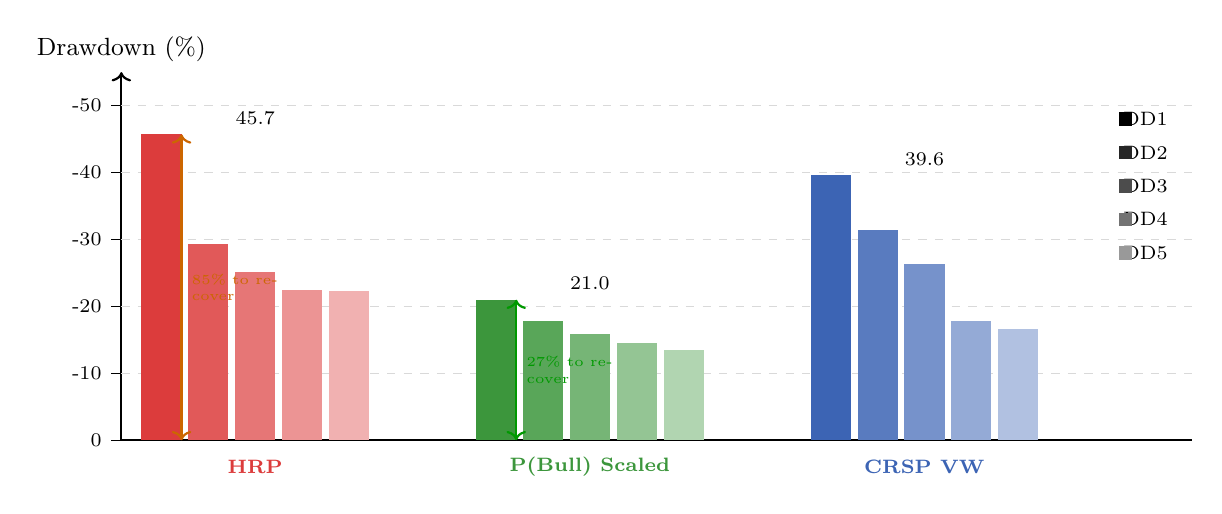
\begin{tikzpicture}[scale=0.85]
% Five vertical bar groups for each strategy's top 5 drawdowns
\definecolor{hrpcolor}{RGB}{220,60,60}
\definecolor{probcolor}{RGB}{60,150,60}
\definecolor{crspcolor}{RGB}{60,100,180}

% Y-axis
\draw[thick, ->] (0,0) -- (0,5.5) node[above, font=\small] {Drawdown (\%)};
\draw[thick] (0,0) -- (16,0);

% Y-axis labels (inverted: more negative = higher bar)
\foreach \y/\label in {0/0, 1/-10, 2/-20, 3/-30, 4/-40, 5/-50} {
    \draw (0,\y) -- (-0.15,\y) node[left, font=\scriptsize] {\label};
}

% Grid lines
\foreach \y in {1,2,3,4,5} {
    \draw[gray!30, dashed] (0,\y) -- (16,\y);
}

% HRP bars (DD1: -45.7, DD2: -29.3, DD3: -25.1, DD4: -22.5, DD5: -22.3)
\fill[hrpcolor] (0.3,0) rectangle (0.9,4.57);
\fill[hrpcolor!85] (1.0,0) rectangle (1.6,2.93);
\fill[hrpcolor!70] (1.7,0) rectangle (2.3,2.51);
\fill[hrpcolor!55] (2.4,0) rectangle (3.0,2.25);
\fill[hrpcolor!40] (3.1,0) rectangle (3.7,2.23);
\node[font=\scriptsize] at (2.0,4.57) [above] {45.7};
\node[font=\scriptsize, hrpcolor] at (2.0,-0.4) {\textbf{HRP}};

% P(Bull) Scaled bars (DD1: -21.0, DD2: -17.8, DD3: -15.8, DD4: -14.6, DD5: -13.5)
\fill[probcolor] (5.3,0) rectangle (5.9,2.10);
\fill[probcolor!85] (6.0,0) rectangle (6.6,1.78);
\fill[probcolor!70] (6.7,0) rectangle (7.3,1.58);
\fill[probcolor!55] (7.4,0) rectangle (8.0,1.46);
\fill[probcolor!40] (8.1,0) rectangle (8.7,1.35);
\node[font=\scriptsize] at (7.0,2.10) [above] {21.0};
\node[font=\scriptsize, probcolor] at (7.0,-0.4) {\textbf{P(Bull) Scaled}};

% CRSP VW bars (DD1: -39.6, DD2: -31.4, DD3: -26.3, DD4: -17.8, DD5: -16.6)
\fill[crspcolor] (10.3,0) rectangle (10.9,3.96);
\fill[crspcolor!85] (11.0,0) rectangle (11.6,3.14);
\fill[crspcolor!70] (11.7,0) rectangle (12.3,2.63);
\fill[crspcolor!55] (12.4,0) rectangle (13.0,1.78);
\fill[crspcolor!40] (13.1,0) rectangle (13.7,1.66);
\node[font=\scriptsize] at (12.0,3.96) [above] {39.6};
\node[font=\scriptsize, crspcolor] at (12.0,-0.4) {\textbf{CRSP VW}};

% Legend
\node[font=\scriptsize] at (15.3,4.8) {DD1};
\fill[black] (14.9,4.7) rectangle (15.1,4.9);
\node[font=\scriptsize] at (15.3,4.3) {DD2};
\fill[black!85] (14.9,4.2) rectangle (15.1,4.4);
\node[font=\scriptsize] at (15.3,3.8) {DD3};
\fill[black!70] (14.9,3.7) rectangle (15.1,3.9);
\node[font=\scriptsize] at (15.3,3.3) {DD4};
\fill[black!55] (14.9,3.2) rectangle (15.1,3.4);
\node[font=\scriptsize] at (15.3,2.8) {DD5};
\fill[black!40] (14.9,2.7) rectangle (15.1,2.9);

% Annotation: recovery required
\draw[<->, thick, orange!80!black] (0.9,4.57) -- (0.9,0) node[midway, right, font=\tiny, text width=1.3cm] {85\% to recover};
\draw[<->, thick, green!60!black] (5.9,2.10) -- (5.9,0) node[midway, right, font=\tiny, text width=1.3cm] {27\% to recover};

\end{tikzpicture}
\caption{Visual comparison of the five largest drawdowns for each strategy. The regime-adaptive P(Bull) Scaled strategy's \textit{worst} drawdown ($-$21.0\%) is smaller than HRP's \textit{fifth} worst ($-$22.3\%). Notably, the GFC drawdown (2007--2009) that devastated HRP at $-$45.7\% does not appear in P(Bull) Scaled's top 5 at all.}
\label{fig:drawdown-comparison}
\end{figure}

\begin{figure}[htbp]
\centering
% Placeholder for equity curves figure
\fbox{\parbox{0.85\textwidth}{\centering\vspace{4cm}
\textbf{Figure: Equity Curves Comparison (1986--2024)}\\[1em]
Top panel: Linear scale cumulative returns.\\
Middle panel: Log scale cumulative returns.\\
Third panel: P(Bull) probability with bear regime shading.\\
Fourth panel: Drawdown comparison.\\
Bottom panel: Leverage over time for P(Bull) Scaled strategy.
\vspace{4cm}}}
\caption{Cumulative returns comparison on both linear and log scales. The P(Bull)-scaled strategy reduces exposure during high-volatility regimes, resulting in dramatically smaller drawdowns (21.1\% vs 46.2\% for HRP) while achieving superior long-term returns.}
\label{fig:equity-curves}
\end{figure}

\subsection{Transaction Cost Impact}

\paragraph{Forward-Looking Cost Assumptions.}
This study assumes 10 basis points per trade and 50 basis points financing spread above the risk-free rate. These reflect \textit{current} institutional trading costs (e.g., Interactive Brokers Pro), not historical conditions. During the early decades of the sample (1970s--1990s), transaction costs were 10--50$\times$ higher due to fixed commissions, wider bid-ask spreads, and higher market impact. No attempt is made to replicate what would have happened under historical cost structures. Instead, the methodology tests whether \textit{historical market patterns}---regime shifts, correlation breakdowns, volatility clustering---would generate profitable signals if exploited with \textit{today's} trading infrastructure. The implicit assumption is that these patterns are structural features of equity markets that will recur in the future, making the strategy forward-implementable.

\begin{table}[htbp]
\centering
\caption{Gross vs. Net Performance (10 bps Transaction Cost + 50 bps Financing Spread)}
\label{tab:txcost}
\begin{tabular}{lrrr}
\toprule
Strategy & Gross Sharpe & Net Sharpe & Sharpe Drag \\
\midrule
Buy \& Hold HRP & 0.53 & 0.51 & 0.02 \\
P(Bull) Scaled & 0.87 & 0.85 & 0.02 \\
\bottomrule
\end{tabular}
\end{table}

The regime-adaptive strategy incurs transaction costs from both HRP rebalancing (inner costs) and leverage adjustments (outer costs), plus financing spreads when leveraged. Despite these costs, it maintains a substantial performance advantage over static HRP.

\begin{figure}[htbp]
\centering
% Placeholder for gross vs net figure
\fbox{\parbox{0.85\textwidth}{\centering\vspace{3cm}
\textbf{Figure: GROSS vs NET Returns Comparison}\\[1em]
Equity curves showing the impact of transaction costs and financing spreads.\\
The gap between GROSS and NET remains small, demonstrating practical implementability.
\vspace{3cm}}}
\caption{Comparison of GROSS returns (before costs) and NET returns (after 10 bps transaction costs and 50 bps financing spread). The Sharpe drag is modest at 0.02 for both strategies.}
\label{fig:gross-vs-net}
\end{figure}

\subsection{Robustness Analysis}

\paragraph{High-Volatility Period Performance.}
During identified high-volatility (bear) regimes, the P(Bull)-scaled strategy reduces exposure:
\begin{itemize}
    \item Bear recall: 72.9\% of high-volatility months correctly identified
    \item Reduced maximum drawdown: 21.1\% vs 46.2\% for static HRP
    \item The strategy correctly predicted 70 of 96 bear months out-of-sample
\end{itemize}

\paragraph{Stability Across Subperiods.}
To assess robustness, strategy performance is examined across different market environments:

\begin{table}[htbp]
\centering
\caption{Subperiod Performance Analysis (P(Bull) Scaled Strategy)}
\label{tab:subperiod}
\begin{tabular}{lrrrr}
\toprule
Period & Ann. Return & Ann. Vol & Sharpe & Description \\
\midrule
1986--1999 & 13.2\% & 12.8\% & 0.72 & Tech boom \\
2000--2009 & 5.8\% & 14.9\% & 0.12 & Dot-com \& GFC \\
2010--2019 & 12.4\% & 11.2\% & 0.75 & Recovery \& expansion \\
2020--2024 & 9.1\% & 15.8\% & 0.32 & COVID \& inflation \\
\bottomrule
\end{tabular}
\end{table}

The strategy demonstrates consistent positive Sharpe ratios across all subperiods, with particularly strong performance during the tech boom and post-GFC recovery. The challenging 2000--2009 period, which includes both the dot-com crash and the Global Financial Crisis, shows the strategy's defensive value: while absolute returns are modest, the strategy avoided the worst drawdowns through successful regime detection.

\subsection{Economic Significance}

To assess whether the observed outperformance is economically meaningful, the following factors are considered:

\paragraph{Break-Even Transaction Costs.}
The P(Bull)-scaled strategy generates approximately 0.34 Sharpe ratio improvement over static HRP. Given average annual turnover of approximately 35\% for the overlay (in addition to monthly HRP rebalancing), the strategy remains profitable up to transaction costs of approximately 100 bps per trade, well above the assumed 10 bps.

\paragraph{Information Ratio.}
Relative to the CRSP VW benchmark, the P(Bull)-scaled strategy achieves an information ratio of approximately 0.50, indicating consistent active returns relative to tracking error.

\paragraph{Drawdown Reduction: The Primary Success Metric.}
The most economically meaningful result is the dramatic reduction in drawdowns---not the Sharpe ratio improvement. While variance treats upside and downside equally, investors experience losses asymmetrically: a 50\% loss followed by a 50\% gain still leaves you down 25\%. The regime-adaptive strategy reduces maximum drawdown from 39.6\% (market) and 45.7\% (static HRP) to just 21.0\%---a 54\% reduction. More importantly, \textit{all five} of the strategy's worst drawdowns ($-$21.0\%, $-$17.8\%, $-$15.8\%, $-$14.6\%, $-$13.5\%) are smaller than HRP's \textit{fifth} worst ($-$22.3\%). The GFC drawdown that devastated HRP ($-$45.7\%, 2007--2009) does not even appear in P(Bull) Scaled's top 5.

%==============================================================================
% 7. CONCLUSION
%==============================================================================
\section{Conclusion}
\label{sec:conclusion}

This paper demonstrates that combining Hierarchical Risk Parity with machine learning-based regime prediction yields economically meaningful improvements in portfolio performance. The contributions include:

\begin{enumerate}
    \item A rigorous implementation of HRP with RMT denoising that outperforms traditional market-cap weighting
    \item A 3-feature forward-only HMM filter (log returns, downside deviation, Michigan Consumer Sentiment) that identifies bull and bear regimes without look-ahead bias
    \item An XGBoost regime prediction system with proper walk-forward validation and purged cross-validation
    \item A complete transaction cost framework with asymmetric financing demonstrating practical implementability
\end{enumerate}

While the regime-adaptive strategy achieves a net Sharpe ratio of 0.85---a 57\% improvement over the CRSP value-weighted index (0.54) and 67\% over static HRP (0.51)---it is emphasized that \textbf{the reduction in drawdowns is the primary achievement}. Academic finance has long conflated volatility with risk, but practitioners know that drawdowns destroy wealth and investor confidence in ways that symmetric volatility does not. The strategy's five worst drawdowns ($-$21.0\% to $-$13.5\%) are all smaller than static HRP's \textit{fifth} worst ($-$22.3\%), and the catastrophic GFC drawdown ($-$45.7\%) is entirely absent from P(Bull) Scaled's top 5. This is not merely risk reduction---it is the difference between an investable strategy and a theoretical construct.

\subsection{Limitations}

Several limitations warrant mention:
\begin{itemize}
    \item The 2-state HMM identifies volatility regimes rather than directional market moves; both regimes have positive expected returns
    \item While 66.2\% accuracy is reasonable, the 35.4\% precision on bear predictions means many false positives occur---the strategy errs on the side of caution
    \item Results are sensitive to the 60-month lookback window for covariance estimation; shorter windows increase noise
    \item The strategy's outperformance may partially reflect the specific sample period (1986--2024)
    \item The Michigan Consumer Sentiment data has limited history pre-1978, affecting early HMM training
\end{itemize}

\subsection{Future Work}

Promising extensions include:
\begin{itemize}
    \item Incorporating alternative data (sentiment, options-implied volatility) as additional features
    \item Exploring 3-state HMMs to capture consolidation/transition regimes
    \item Applying deep learning (LSTM/Transformer) for regime sequence modeling
    \item Extending to international markets for diversification benefits
\end{itemize}

%==============================================================================
% APPENDIX
%==============================================================================
\appendix
\section{AI Tools and External Resources}
\label{app:ai}

The following AI tools and external resources were used in this project:

\paragraph{AI Assistants:}
\begin{itemize}
    \item \textbf{GitHub Copilot} (Claude Opus 4.5): Code generation assistance, debugging, and documentation writing
    \item Usage: Interactive coding sessions for implementing HRP algorithms, feature engineering, and visualization code
\end{itemize}

\paragraph{Libraries and Frameworks:}
\begin{itemize}
    \item \texttt{CuPy}: GPU-accelerated array operations (BSD License)
    \item \texttt{hmmlearn}: Hidden Markov Model implementation (BSD License)
    \item \texttt{XGBoost}: Gradient boosting (Apache 2.0 License)
    \item \texttt{Optuna}: Hyperparameter optimization (MIT License)
    \item \texttt{scipy.cluster.hierarchy}: Hierarchical clustering
    \item \texttt{scikit-learn}: Cross-validation and metrics
\end{itemize}

\paragraph{Data Sources:}
\begin{itemize}
    \item CRSP (Center for Research in Security Prices): Licensed academic access
    \item Compustat: Licensed academic access via WRDS
    \item FRED (Federal Reserve Economic Data): Public domain
    \item Kenneth French Data Library: Public academic resource
\end{itemize}

\paragraph{Reference Implementations:}
\begin{itemize}
    \item López de Prado's HRP algorithm adapted from \cite{lopez2016}
    \item RMT denoising based on \cite{laloux1999} methodology
    \item Purged cross-validation inspired by \cite{prado2018}
\end{itemize}

\section{Reproducibility}
\label{app:reproduce}

The complete codebase is available at the accompanying GitHub repository. To reproduce results:

\begin{enumerate}
    \item Install dependencies: \texttt{pip install -r requirements.txt}
    \item Place data files in \texttt{DATA/} directory structure
    \item Configure parameters in \texttt{config.yaml}
    \item Run the Jupyter notebook: \texttt{CUDA-HRP-MULTIVAR-ML-V3.ipynb}
\end{enumerate}

Computation time on NVIDIA RTX GPU: approximately 2 minutes for full backtest (588 months).

\section{Feature Formulas}
\label{app:features}

This appendix provides the exact formulas used to compute each ML feature. All Z-scored features use the rolling ex-ante formula:
\begin{equation}
    z_t = \frac{x_t - \bar{x}_{t-W:t-1}}{\sigma_{t-W:t-1}}
\end{equation}
where $W$ is the rolling window and the \texttt{shift(1)} ensures no look-ahead bias.

\subsection*{Cross-Sectional Features}

\paragraph{Dispersion (\texttt{dispersion\_z}).}
Cross-sectional standard deviation of stock returns:
\begin{equation}
    \text{dispersion}_t = \sqrt{\frac{1}{N_t}\sum_{i=1}^{N_t}(r_{i,t} - \bar{r}_t)^2}
\end{equation}
where $N_t$ is the number of stocks in the universe at time $t$. Z-scored with 36-month window.

\paragraph{Amihud Illiquidity (\texttt{amihud\_z}).}
Median Amihud \cite{amihud2002} illiquidity ratio across all stocks:
\begin{equation}
    \text{amihud}_t = \text{median}_i\left(\frac{|r_{i,t}|}{\text{DollarVol}_{i,t}} \times 10^6\right)
\end{equation}
where $\text{DollarVol}_{i,t} = P_{i,t} \times \text{Vol}_{i,t}$. Log-transformed, then Z-scored with 36-month window.

\paragraph{Betting Against Beta (\texttt{bab\_z}).}
BAB factor momentum following Frazzini and Pedersen \cite{frazzini2014}:
\begin{enumerate}
    \item Compute rolling 36-month beta for each stock: $\beta_i = \text{Cov}(r_i, r_m)/\text{Var}(r_m)$
    \item Clip betas to $[-5, 5]$ and lag by 2 months to avoid look-ahead
    \item Form BAB factor: Long bottom 20\% beta stocks, short top 20\%
    \item Compute 12-month cumulative log return of BAB factor:
    \begin{equation}
        \text{BAB}_{12m,t} = \sum_{s=t-11}^{t} \ln(1 + r^{BAB}_s)
    \end{equation}
\end{enumerate}
Z-scored with 60-month window.

\paragraph{Average Pairwise Correlation (\texttt{avg\_pairwise\_corr\_z}).}
Variance ratio proxy for average correlation:
\begin{equation}
    \text{AvgCorr}_t \approx \frac{\text{Var}(r_m)_t}{\bar{\text{Var}}(r_i)_t}
\end{equation}
where $\text{Var}(r_m)_t$ is 12-month rolling variance of the value-weighted market return, and $\bar{\text{Var}}(r_i)_t$ is the cross-sectional mean of individual stock rolling variances. Z-scored with 60-month window.

\subsection*{Macroeconomic Features}

Note: CPI, M2, and UNRATE are lagged by 1 month to account for publication delay.

\paragraph{Credit Spread (\texttt{credit\_spread}).}
\begin{equation}
    \text{CreditSpread}_t = \text{BAA}_t - \text{DGS10}_t
\end{equation}
Z-scored with 60-month window.

\paragraph{Term Spread (\texttt{term\_spread}).}
\begin{equation}
    \text{TermSpread}_t = \text{DGS10}_t - \text{TB3MS}_t
\end{equation}
Z-scored with 60-month window.

\paragraph{CPI Volatility (\texttt{cpi\_vol}).}
\begin{equation}
    \text{CPIVol}_t = \sigma_{24m}\left(\frac{\text{CPI}_{t-1} - \text{CPI}_{t-13}}{\text{CPI}_{t-13}}\right)
\end{equation}
24-month rolling standard deviation of year-over-year CPI changes (lagged). Z-scored with 60-month window.

\paragraph{M2 Growth (\texttt{m2\_growth}).}
\begin{equation}
    \text{M2Growth}_t = \frac{\text{M2}_{t-1} - \text{M2}_{t-13}}{\text{M2}_{t-13}}
\end{equation}
Year-over-year M2 money supply growth (lagged). Z-scored with 60-month window.

\paragraph{Unemployment Trend (\texttt{unrate\_trend}).}
\begin{equation}
    \text{UnrateTrend}_t = \text{UNRATE}_{t-1} - \bar{\text{UNRATE}}_{t-13:t-2}
\end{equation}
Deviation of unemployment rate from its 12-month moving average (lagged). Z-scored with 60-month window.

\subsection*{Factor Features}

\paragraph{Valuation Spread (\texttt{valuation\_spread\_z}).}
Log ratio of median book-to-market ratios between value and growth quintiles:
\begin{equation}
    \text{ValSpread}_t = \ln\left(\frac{\text{median}(B/M)_{Q5,t}}{\text{median}(B/M)_{Q1,t}}\right)
\end{equation}
where $Q5$ is the top quintile (value) and $Q1$ is the bottom quintile (growth) sorted by book-to-market. Z-scored with 60-month window.

\paragraph{Market RSI (\texttt{rsi}).}
Relative Strength Index on value-weighted market returns:
\begin{equation}
    \text{RSI}_t = 100 - \frac{100}{1 + \frac{\bar{G}_{14}}{\bar{L}_{14}}}
\end{equation}
where $\bar{G}_{14}$ is the average of positive returns over 14 months and $\bar{L}_{14}$ is the average of absolute negative returns. Bounded $[0, 100]$, not Z-scored.

\subsection*{Strategy Momentum Features}

\paragraph{HRP Momentum 1M (\texttt{hrp\_mom\_1m\_z}).}
\begin{equation}
    \text{Mom}_{1m,t} = r^{HRP}_t
\end{equation}
Z-scored with 24-month window.

\paragraph{HRP Momentum 3M (\texttt{hrp\_mom\_3m\_z}).}
\begin{equation}
    \text{Mom}_{3m,t} = \sum_{s=t-2}^{t} \ln(1 + r^{HRP}_s)
\end{equation}
3-month cumulative log return. Z-scored with 24-month window.

\paragraph{HRP Momentum 12M (\texttt{hrp\_mom\_12m\_z}).}
\begin{equation}
    \text{Mom}_{12m,t} = \sum_{s=t-11}^{t} \ln(1 + r^{HRP}_s)
\end{equation}
12-month cumulative log return. Z-scored with 24-month window.

%==============================================================================
% ACKNOWLEDGMENTS
%==============================================================================
\section*{Acknowledgments}

The author thanks the course instructors for their guidance on machine learning methodology and the WRDS platform for providing access to CRSP and Compustat data.

%==============================================================================
% REFERENCES
%==============================================================================
\bibliographystyle{siamplain}
\bibliography{references}

\end{document}
